\begin{chapter}{Algoritmi disponibili}
\label{sec:algoritmi}

In ANT sono stati implementati due tipi di algoritmi di ricerca:
\begin{itemize}
	\item Ricerca non informata (o a \textit{tentativi} o anche \textit{cieca})
	\item Ricerca informata
\end{itemize}

Queste due tipologie di ricerca differiscono per la presenza, nella ricerca
informata, di una \textbf{funzione euristica} che non fa altro che fornire una
stima della distanza dall'obiettivo tramite una rappresentazione matematica della
conoscenza del problema. Per esempio, nel problema classico del gioco dell'otto,
la nostra funzione euristica potrebbe essere una funzione che conta il numero di
caselle fuoriposto rispetto alla configurazione finale. Tale funzione \`e quella
descritta durante la descrizione del blocco delle euristiche in \ref{sec:heuristic-block}.
Analizzeremo, comunque, questo caso pi\`u nello specifico in \ref{sec:heuristicdef}.

La scelta di un algoritmo rispetto ad un altro e, intrinsecamente, lo studio
dell'algoritmo in s\'e per s\'e si basa su quattro fattori:

\begin{enumerate}
	\item \textbf{completezza}: la garanzia di trovare una soluzione valida per
        il problema in esame, se esiste
	\item \textbf{complessit\`a temporale}: il tempo richiesto dall'algoritmo per
        risolvere il problema
	\item \textbf{complessit\`a spaziale}: la quantit\`a di memoria richiesta
        dall'algoritmo per risolvere il problema
  \item \textbf{ottimalit\`a}: la garanzia di trovare la soluzione \textit{ottima}
        nel caso esistano pi\`u soluzioni per lo stesso problema (es: trovare il
        percorso minimo tra due citt\`a),
\end{enumerate}

Gli algoritmi implementati mostrano diverse caratteristiche per ognuno di questi
fattori. Per i dettagli relativi a completezza, complessit\`a temporale e spaziale
e ottimalit\`a di ogni singolo algoritmo si rimanda a \cite{norvig03} che fornisce
una discussione approfondita sia dell'algoritmo in s\'e per s\'e che un'analisi di
tutti i fattori sopra descritti relativamente all'algoritmo in questione.

I metodi di ricerca non informati si basano sulla possibilit\`a di esplorazione
dell'intero spazio di ricerca. Come \`e facile intuire, spesso l'ampiezza dello
spazio di ricerca \`e estremamente ampia e questi algoritmi risultano inapplicabili
sia in termini di complessit\`a temporale che spaziale.

Per velocizzare l'applicazione degli algoritmi ed evitare l'ingresso in cammini
ciclici (ovvero da un nodo si genera il suo genitore, quindi si ripete il ciclo
all'infinito) oppure gi\`a considerati, durante la generazione di ogni nuovo nodo
nell'albero di ricerca viene controllato se il nodo in questione \`e stato gi\`a
generato. Questa verifica \`e fatta creando, per ogni nodo generato, un hash della
sua rappresentazione ed inserendo tale rappresentazione in un \verb,set,. In questo
modo, la ricerca di un hash precedentemente calcolato ha complessit\`a $O(1)$.

La discussione dei due algoritmi di ricerca non informata implementati, ovvero
ricerca in ampiezza (\textit{Breadth First Search} o \textit{BFS}) e ricerca in
profondit\`a (\textit{Depth First Search} o \textit{DFS}) segue rispettivamente
in \ref{sec:non-informed-algos} mentre i due algoritmi di ricerca informata A* e
Hill climbing sono discussi in \ref{sec:informed-algos}.

Nei capitoli che seguono, il problema di riferimento \`e quello del gioco dell'8
che viene illustrato in appendice \ref{sec:gioco-filetto}.

\begin{section}{Algoritmi di ricerca non informata}
\label{sec:non-informed-algos}
Come gi\`a detto in precedenza, gli algoritmi di ricerca non informati si basano
sulla possibilit\`a di esplorare l'intero spazio di ricerca. Questo, per\`o, potrebbe
non essere sempre possibile per diversi motivi:

\begin{itemize}
    \item lo spazio di ricerca \`e particolarmente ampio: potrebbe succedere che
    il problema in questione ha uno spazio di ricerca troppo grande per essere
    totalmente esplorato. Il gioco dell'8 ne \`e un esempio, difatti teoricamente
    l'albero ha profondit\`a infinita essendo possibile spostare il tassello e poi
    riportarlo nella sua posizione precedente e continuando cos\`i all'infinito.
    Questo problema pu\`o essere minimizzato evitando le ripetizioni di stati,
    evitando di fatto di ripercorrere cammini gi\`a analizzati.
    \item non abbiamo la certezza che la soluzione esista: questo significa che
    potrebbe succedere di esplorare tutto lo spazio di ricerca senza per\`o
    arrivare ad uno stato finale per il problema in questione (questo non \`e
    valido per il gioco dell'8 in quanto, se la configurazione di partenza \`e
    una configurazione valida, allora sicuramente questa porter\`a ad uno stato
    finale accettabile).
\end{itemize}

In ANT \`e possibile definire un limite tramite la clausola \verb,limit, descritta in
\ref{sec:option-block} che impone un limite sulla profondit\`a raggiungibile dall'albero
delle soluzioni. In questo modo, tutte le configurazioni con una profondit\`a maggiore o
uguale del limite imposto verranno ignorate. Tale limite si dimostra particolarmente
utile durante l'applicazione del DFS.

	\begin{subsection}{Breadth-First search}
    Il \textit{Breadth-First search} o \textit{BFS} effettua una ricerca in ampiezza
    sull'albero delle soluzioni. Partendo dalla configurazione iniziale (livello 0 o radice),
    genera tutte le possibili configurazioni successive (livello 1). Dopodich\'e
    per ogni nodo del livello 1, genera tutte le sue configurazioni successive (livello
    2) e cos\`i via sino a quando viene riconosciuta una configurazione finale
    valida oppure non \`e possibile continuare, ossia non ci sono altre configurazioni
    generabili oppure tutte quelle generabili sono state gi\`a percorse.

    Questo modo di procedere ci assicura che se almeno una soluzione esiste, verr\`a
    trovata, ed in particolar modo verr\`a trovata quella col il cammino pi\`u breve.

    \begin{figure}[!htb]
        \centering
        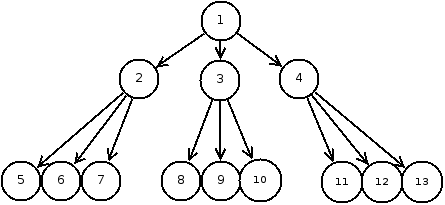
\includegraphics[scale=0.5]{img/bfs.png}
        \caption{Ordine di espansione dei nodi nel BFS}
        \label{fig:bfs-tree}
    \end{figure}

    Bisogna tuttavia notare che questo algoritmo \`e applicabile nel caso in cui il
    grafo, che nel nostro caso \`e implicito, non sia pesato. Questo \`e sempre vero
    nel nostro caso, dato che assumiamo che la generazione di un nuovo nodo non abbia
    peso (in realt\`a questa \`e un'assunzione che facciamo solo nel caso degli algoritmi
    non informati). Nel caso si disponga di un grafo pesato, \`e possibile utilizzare
    algoritmi pi\`u complessi come quello per la ricerca del cammino minimo in un grafo
    di Dijkstra \cite{Skiena08}.

    L'applicazione di questo algoritmo ha senso per determinate istanze del gioco dell'8,
    in quanto le configurazioni generabili da ogni nodo possono essere al massimo quattro
    nel caso in cui il tassello vuoto si trovi al centro del quadrato di gioco, potendosi
    quindi muovere in su, in gi\`u, a destra ed a sinistra. Inoltre, la profondit\`a
    dell'albero da generare dipende dal numero di mosse minime richieste per risolvere la
    particolare istanza del problema. Un'istanza che richiede un minimo di cinque mosse per
    raggiungere la configurazione finale avr\`a difatti un albero di profondit\`a cinque. 
    Dunque, se la profondit\`a dell'albero \`e limitata, cio\'e il gioco \`e risolvibile
    in poche mosse, allora il BFS \`e un algoritmo accettabile\footnote{per accettabile si
    intende computazionalmente possibile in termini di tempo/risorse necessarie per risolvere
    il gioco.} per il gioco dell'8.
	\end{subsection}

	\begin{subsection}{Depth-First search}
    Il \textit{Depth-First search} o \textit{DFS}, al contrario del BFS, effettua una
    ricerca in profondit\`a sull'albero delle soluzioni. Ci\`o significa che, partendo
    dalla configurazione iniziale (livello 0 o radice), genera tutte le possibili
    configurazioni successive. Dopodich\'e prende il primo figlio generato e lo
    considera come una nuova radice e ripete l'operazione. Questo porta ad esplorare
    tutti i cammini che passano da una determinata configurazione, fermandosi solo quando
    si raggiunge una configurazione finale valida oppure non ci sono pi\`u nodi generabili.
    Nel caso si dovessero verificare una delle due condizioni ora citate si ritorna al
    nodo genitore e si procede con l'esplorazione di un cammino alternativo.

    \begin{figure}[!htb]
        \centering
        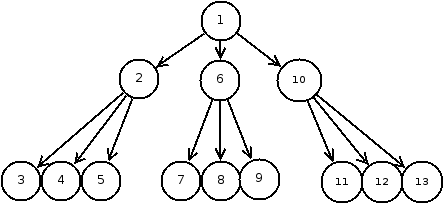
\includegraphics[scale=0.5]{img/dfs.png}
        \caption{Ordine di espansione dei nodi nel DFS}
        \label{fig:dfs-tree}
    \end{figure}
	\end{subsection}

    Il DFS non da nessuna garanzia sul ritrovamento di una soluzione ottima n\'e
    ottimale, ma ci garantisce che, se almeno una soluzione esiste, sar\`a trovata.
    \`E possibile infatti che il DFS trovi una soluzione qualunque piuttosto che
    trovare la soluzione ottima (cosa che non succede, invece, col BFS).

    L'utilizzo del DFS \`e utile nei casi in cui la profondit\`a dell'albero generato
    non sia eccessiva, ossia in problemi in cui siano possibili un numero limitato
    di \textit{mosse} a partire da ogni determinata configurazione. A prova di ci\`o
    si segnala l'inadeguatezza del DFS per il gioco dell'8, comprovata dalle tabelle
    in \ref{tbl:confronto-algoritmi}. In questo specifico problema, per ogni configurazione,
    sono disponibili sempre almeno due mosse\footnote{a meno che queste due mosse non
    portino a configurazioni gi\`a generate in precedenza e che quindi non avrebbe senso
    ripetere}, pertanto ogni nodo pu\`o generare sempre, con le dovute considerazioni,
    almeno due ulteriori cammini.
\end{section}

\begin{section}{Algoritmi di ricerca informata}
\label{sec:informed-algos}

Gli algoritmi di ricerca informata si basano sulla disponibilit\`a di una \textit{funzione
euristica}, ovvero di una funzione matematica in grado di fornire una stima della distanza
di una particolare configurazione dall'obiettivo.
La presenza di tale funzione permette a questo genere di algoritmi di risolvere alcuni
problemi senza aver bisogno di esplorare tutto lo spazio di ricerca che, come gi\`a affermato
pi\`u volte, pu\`o essere talmente ampio da rendere praticamente impossibile, dal punto vista
di risorse necessarie, la sua totale esplorazione. Per una spiegazione dettagliata
sull'utilit\`a delle funzioni euristiche e sulla loro ammissibilit\`a (in semplici parole, un
euristica ammissibile non sbaglia mai per eccesso la stima del costo per raggiungere
l'obiettivo) si rimanda a \cite{norvig03}.

    \begin{subsection}{Definizione della funzione euristica}
    \label{sec:heuristicdef}
    Una funzione euristica deve fornire una stima, in termini numerici, della distanza
    dall'obiettivo. Chiaramente ci\`o dipende dal problema in oggetto, pertanto ANT mette a
    disposizione la possibilit\`a di definire una o pi\`u funzioni euristiche.
    Una funzione euristica in ANT si definisce tramite il blocco \verb,beginHeuristic,-\verb,endHeuristic,
    di cui si pu\`o trovare una descrizione formale in \ref{sec:heuristic-block}.

    Ad esempio per il gioco dell'otto abbiamo individuato due possibili funzioni euristiche:
    \begin{itemize}
        \item una funzione semplice che consiste nel contare il numero di tasselli non in
        posizione corretta. L'idea alla base \`e che tanti pi\`u tasselli saranno fuori posto
        tanto pi\`u distante sar\`a l'obiettivo.
        Sia $pos(x, C)$ la funzione che ritorna $1$ se il tassello $x$ non \`e in posizione corretta
        per la configurazione $C$ e $0$ altrimenti, allora la funzione euristica sar\`a definita come
        $h(n, C) = \sum_{i=1}^{8}{pos(i, C)}$ ove $n$ \`e il nodo che stiamo considerando. Ad esempio,
        per la seguente configurazione il valore ritornato dalla funzione euristica sar\`a $4$.

        \begin{center}
        \begin{tabular}{| c | c | c |}
        \hline
        8 & 1 & 3\\\hline
        7 &   & 4\\\hline
        6 & 2 & 5\\\hline
        \end{tabular}
        \end{center}

        \item la distanza di Manhattan, che consiste nel sommare, per ogni tassello, il numero
        di operazioni necessarie per portarlo in posizione corretta. Come si pu\`o intuire,
        questa funzione consente una valutazione molto pi\`u precisa di quella dei
        tasselli mancanti. Per la stessa configurazione vista precedentemente, la distanza di
        Manhattan sar\`a $5$.
    \end{itemize}

    Si pu\`o notare che i valori ritornati dalle due euristiche, a parit\`a di configurazione,
    sono diversi. In particolare, la distanza di Manhattan considera la stessa configurazione
    pi\`u \textit{lontana} dall'obiettivo rispetto all'euristica dei tasselli fuori posto.
    \end{subsection}

    \begin{subsection}{A*}
    Sia $g(n)$ la funzione che ritorna il costo del cammino dal nodo iniziale al nodo $n$ (in ANT
    tale valore \`e l'indice della profondit\`a del nodo, ovvero il numero di nodi da attraversare
    a partire dalla radice per raggiungere il nodo $n$) ed $h(n)$ la funzione euristica per il
    problema in questione, allora la funzione $f(n) = g(n) + h(n)$ fornir\`a una valutazione della
    distanza del nodo su cui viene applicata dall'obiettivo.

    Per ogni nodo dell'albero delle soluzioni, A* genera tutti i suoi possibili successori applicando
    la $f(n)$ su di essi e memorizzandone il valore risultante come costo associato per raggiungere
    l'obiettivo. Tali nodi vengono inseriti in una coda con priorit\`a ordinata in base al costo
    precedentemente calcolato; allora il successivo nodo da espandere sar\`a l'elemento in cima alla
    coda con priorit\`a.

    Una volta raggiunto l'obiettivo, si procede a ritroso verso il nodo radice per individuare il
    cammino seguito. Tale cammino sar\`a non solo una soluzione del problema, sar\`a anche la
    soluzione ottima. Questo \`e provato dal requisito di ammissibilit\`a della funzione euristica
    introdotto nei capitoli precedenti. La dimostrazione di tale affermazione \`e riportata
    in \cite{norvig03}.
    \end{subsection}

    \begin{subsection}{Hill Climbing}
    L'idea alla base dell'hill climbing \`e quella di seguire sempre il percorso pi\`u promettente.
    Come in A*, quando vengono generati i successori per ogni nodo, viene calcolato il costo
    stimato per raggiungere l'obiettivo tramite la funzione $f(n)$ vista nel capitolo precedente.
    A differenza dell'A* i nodi non vengono inseriti in una coda con priorit\`a, bens\`i viene
    preso il nodo con il costo minore ignorando gli eventuali altri nodi.

    \begin{figure}[!htb]
        \centering
        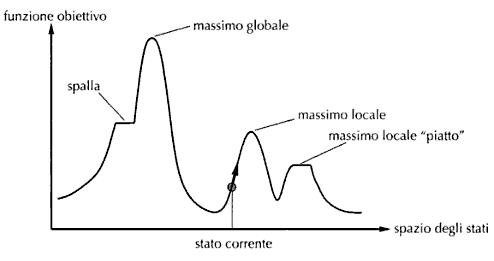
\includegraphics[scale=0.5]{img/hillclimbing.png}
        \caption{Rappresentazione grafica dell'algoritmo di Hill Climbing, fonte \cite{norvig03}}
        \label{fig:hillclimbing}
    \end{figure}

    Si immagina la scalata di una montagna dove, idealmente, la strada pi\`u ripida tra quelle vicine
    \`e quella che permette di raggiungere in minor tempo la cima (obiettivo). Questo pu\`o portare
    alcuni problemi come quelli in figura:
    \begin{itemize}
        \item raggiungendo la \textit{spalla}, sia a destra che a sinistra della posizione corrente
        non si ha n\'e una salita n\'e una discesa. Si pone quindi il problema di dover scegliere
        una delle due direzioni senza avere indicazioni su quale strada sia meglio seguire.
        \item esiste il rischio di raggiungere un \textit{massimo locale}, ovvero si \`e raggiunta
        una cima che per\`o non \`e la soluzione del problema. Sia a destra che a sinistra sono
        presenti strade in discesa che pertanto non vengono considerate.
    \end{itemize}

    \`E possibile evitare questi problemi utilizzando procedure di backtracking nel caso in cui si
    raggiungesse una situazione di stallo, ma nella nostra implementazione abbiamo utilizzato la
    versione nai\"ve dell'algoritmo in cui non prendiamo in considerazione questi problemi. Difatti,
    come si pu\`o vedere in \ref{tbl:confronto-algoritmi-2}, l'algoritmo di hill climbing non
    riesce a trovare una soluzione per il problema del gioco dell'8 al contrario degli altri
    algoritmi.
    \end{subsection}
\end{section}

\begin{section}{Confronto tra gli algoritmi}
Abbiamo scelto un problema classico non banale quale quello del gioco dell'8
e abbiamo messo a confronto i diversi algoritmi descritti nelle sezioni
precedenti. I risultati ottenuti rispettano appieno le nostre aspettative,
difatti gli algoritmi informati si sono dimostrati molto pi\`u veloci di
quelli non informati. Tuttavia, su una piccola istanza del problema (gioco
dell'8 risolvibile in due mosse) gli algoritmi hanno avuto pi\`u o meno
le stesse performance. Questo \`e dovuto al fatto che l'albero di ricerca
in questo caso \`e molto piccolo, pertanto la sua completa esplorazione non
richiede un tempo eccessivo.

\noindent Nella tabella che segue, sono riassunti i risultati che abbiamo ottenuto:

\label{tbl:confronto-algoritmi}

\begin{center}
    \label{tbl:confronto-algoritmi-1}
    \begin{tabular}{| c | c | c | c | c | c |}
    \hline
    \multicolumn{6}{|c|}{\textit{Gioco dell'8 risolvibile in due mosse}} \\
    \hline
                     & A* (1) & A* (2) & Hill climbing & BFS    & DFS     \\\hline
    Tempo di         &        &        &               &        &         \\
    esecuzione       & 0.716s & 0.732s & 1.232s        & 0.808s & 27.421s \\\hline
    Mosse            &        &        &               &        &         \\
    richieste        & 2      & 2      & 2             & 2      & 10      \\\hline
    Memoria          &        &        &               &        &         \\
    occupata         & 3280Kb & 3280Kb & 3280Kb        & 3280Kb & 3664Kb  \\\hline
    Nodi espansi     & 3      & 3      & 2             & 2      & 254     \\\hline
    Limite           &        &        &               &        &         \\
    (se applicabile) & n/a    & n/a    & 10            & 10     & 10      \\\hline
    \end{tabular}
\end{center}

\noindent \\Le due diverse esecuzioni di A* si riferiscono alle due euristiche
descritte in precedenza, in particolare la (1) si riferisce all'euristica della
distanza di Manhattan mentre la (2) si riferisce all'euristica del conteggio dei
tasselli fuoriposto.

Nel confronto successivo \`e stata utilizzata un'istanza del problema pi\`u
complessa per evidenziare le diverse caratteristiche degli algoritmi.
Difatti, nel caso seguente, sono richieste almeno sette mosse per risolvere il problema:

\begin{center}
    \label{tbl:confronto-algoritmi-2}
    \begin{tabular}{| c | c | c | c | c | c |}
    \hline
    \multicolumn{6}{|c|}{\textit{Gioco dell'8 risolvibile in sette mosse}} \\
    \hline
                     & A* (1) & A* (2) & Hill climbing & BFS     & DFS      \\\hline
    Tempo di         &        &        &               &         &          \\
    esecuzione       & 1.956s & 5.963s & 7.244s        & 13.548s & 115.411s \\\hline
    Mosse            &        &        &               &         &          \\
    richieste        & 7      & 7      & n/a           & 7       & 9        \\\hline
    Memoria          &        &        &               &         &          \\
    occupata         & 3280Kb & 3408Kb & 3408Kb        & 3536Kb  & 4944Kb   \\\hline
    Nodi espansi     & 26     & 78     & 21            & 131     & 1167     \\\hline
    Limite           &        &        &               &         &          \\
    (se applicabile) & n/a    & n/a    & 10            & 10      & 12       \\\hline
    \end{tabular}
\end{center}

\noindent \\ Come nel caso precedente, i due A* si riferiscono rispettivamente al
caso in cui viene utilizzata l'euristica della distanza di Manhattan e quello in
cui l'euristica \`e quella del conteggio dei tasselli fuoriposto. Bisogna notare
che l'algoritmo di hill climbing in questo caso non ha saputo trovare una soluzione
al problema.

\end{section}

\end{chapter}
